\documentclass[]{article} 
\usepackage{pgfplots} 
\usepgfplotslibrary{external} 
\tikzexternalize 
\usepgfplotslibrary{fillbetween}
\usepackage{tikz} 
\usepackage{amsmath} 
\usepackage{pgfplots} 
\usetikzlibrary{calc} 
\pgfplotsset{compat = newest, every axis plot post/.style={line join=round}, label style={font=\Large},every tick label/.append style={font=\large}  }
\begin{document} 
	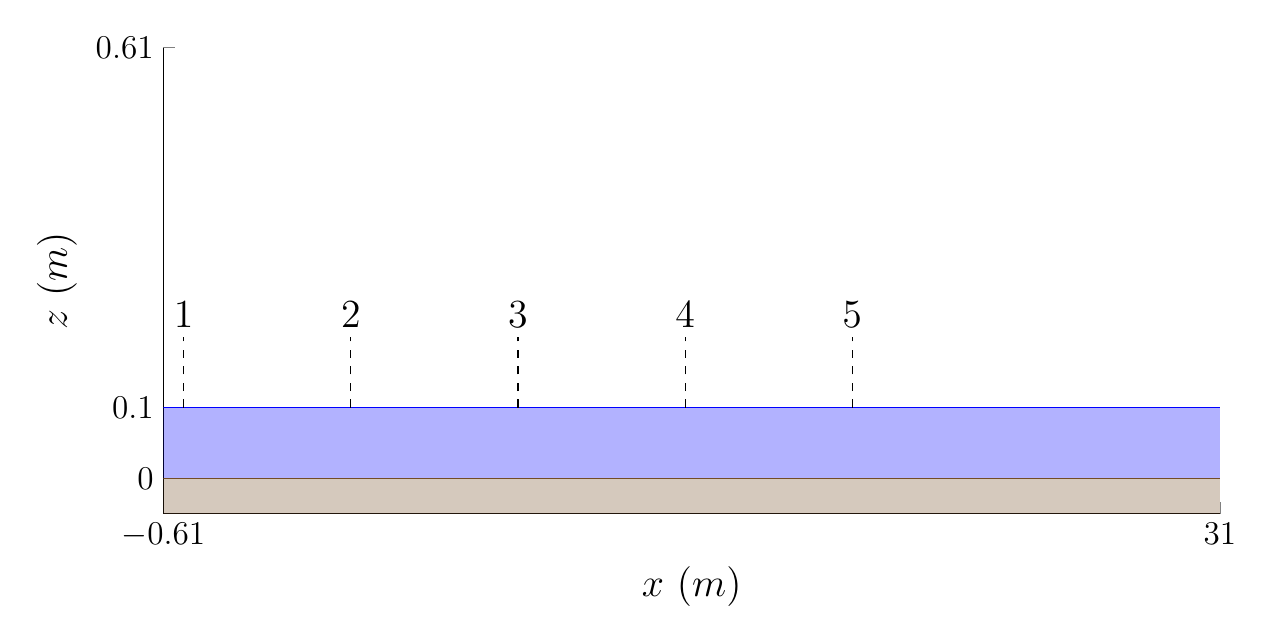
\begin{tikzpicture}
	\begin{axis}[ 
	width = 0.7\textwidth,
	width=15cm,
	height = 7.5cm,
	axis y line*=left,
	axis x line*=bottom, 
	xtick={-0.61,31},  
	ytick = {0,0.1,0.61}, 
	xmin=-0.61, 
	xmax=31, 
	ymin =-0.05, 
	ymax = 0.61,
	xlabel=$x$ ($m$), 
	ylabel=$z$ ($m$)]
	
	\addplot [name path=b,brown!60!black] coordinates {(-0.61,0)  (31.6,0)};
	
	\path[name path=axis] (axis cs:-0.61,-0.05) --  (axis cs:31.6,-0.05);
	
	\addplot [name path=a,blue] coordinates {(-0.61,0.1)  (31.6,0.1)};
	
		\addplot [
		thick,
		color=brown!60!black,
		fill=brown!60!black, 
		fill opacity=0.3
		] fill between[of=b and axis];
		
	\addplot [
	thick,
	color=blue,
	fill=blue, 
	fill opacity=0.3
	] fill between[of=a and b];
	
	
	\addplot [black,dashed] coordinates {(0,0.1) (0,0.2)};
	\node[above] at (axis cs:0,0.2) {\Large$1$};
	
	\addplot [black,dashed] coordinates {(5,0.1) (5,0.2)};
	\node[above] at (axis cs:5,0.2) {\Large$2$};

	\addplot [black,dashed] coordinates {(10,0.1) (10,0.2)};
	\node[above] at (axis cs:10,0.2) {\Large$3$};

	\addplot [black,dashed] coordinates {(15,0.1) (15,0.2)};
	\node[above] at (axis cs:15,0.2) {\Large$4$};
	
	\addplot [black,dashed] coordinates {(20,0.1) (20,0.2)};
	\node[above] at (axis cs:20,0.2) {\Large$5$};
	\end{axis} 
	
	
	
	\end{tikzpicture}
\end{document}